\documentclass{article}

\usepackage[main=english,russian]{babel}
\usepackage[T1]{fontenc}
\usepackage[utf8]{inputenc}
\usepackage[sexy]{evan}
\usepackage{cancel}
\usepackage{matchsticks}
\usepackage{wrapfig}
\usepackage{listings}

\title{Insightful Proofs - Part 1}

\author{Nghia Doan}
\date{\today}

\begin{document}

\maketitle

\begin{example}[Knight Tour and Parity]\label{example:knight-tour-parity}
    A knight stands on square \( A \) of a regular chessboard. Is it possible for the knight to go to square \( B \), visiting each remaining square exactly once on the way?
    \index{Knight Tour} \index{Parity Argument} \index{Chessboard Coloring}
\end{example}

\begin{analysis*}
    At first, it seems like a difficult problem where the only thing we can do is try various knight moves and see if it's possible to reach \( B \) from \( A \). But after a few trials, it becomes clear that it’s not easy to try all possibilities — we must find another approach.

    It’s important in such cases to stop and observe what information is given.
\end{analysis*}

\begin{soln}\ \\\indent
    We are given three key facts:
    \begin{itemize}[topsep=0pt, partopsep=0pt, itemsep=0pt]
        \item A chessboard has 64 squares.
        \item Squares \( A \) and \( B \) are both black.
        \item With every move, a knight goes from a black square to a white square, or vice versa.
    \end{itemize}

    \begin{center}
        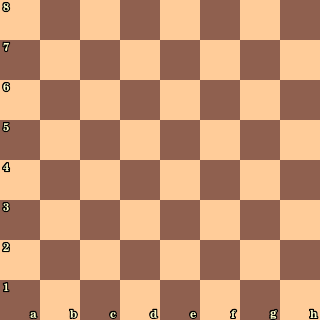
\includegraphics[width=5cm]{./png/chess-board.png}
    \end{center}

    The third fact is crucial. It tells us that the color of the square alternates with every move — just like parity alternates between even and odd: odd, even, odd, even, \(\ldots\)

    \textbf{Note:} This two-value alternation is a form of the \emph{principle of parity}, which we can use to solve many problems.

    Since the knight must visit all 64 squares, it must make exactly \( 63 \) moves. Each move changes the color of the square the knight is on.

    If the knight starts on a black square (say, square \( A \)), then after 63 moves — an odd number — it must land on a square of the opposite color: a white square.

    But square \( B \) is also black. So the knight cannot end up at \( B \).

    Hence, the answer is 
    \(
        \boxed{\text{no, it is not possible.}}
    \)
\end{soln}

\begin{remark*}
    This problem showcases a simple but powerful idea — tracking color alternation, or parity — instead of attempting brute-force paths. Many chessboard problems reduce to identifying such hidden invariants.
\end{remark*}


\begin{example}[Sum of First 10 Odd Integers]\label{example:sum-of-first-10-odd}
    Can you determine the sum of the first 10 odd positive integers without adding them up?
    \index{Odd Numbers} \index{Visual Proof} \index{Arithmetic Sequences}
\end{example}

\begin{analysis*}
    This problem seems numerical at first, but there's a geometric pattern behind it. Instead of brute-force addition, we look for structure — especially using shapes or grouping techniques that simplify the computation.
\end{analysis*}

\begin{soln}[Visual proof with L-shaped blocks]\ \\\indent
    Consider a square of size \( 10 \times 10 \), built up layer by layer using nested L-shapes.

    \begin{center}
        \begin{tabular}{llll
            >{\columncolor[HTML]{F5AE09}}l 
            >{\columncolor[HTML]{A30003}}l 
            >{\columncolor[HTML]{85004C}}l 
            >{\columncolor[HTML]{073A6C}}l 
            >{\columncolor[HTML]{0E6A63}}l 
            >{\columncolor[HTML]{0D6002}}l }
            \cellcolor[HTML]{0D6002} & \cellcolor[HTML]{0D6002} & \cellcolor[HTML]{0D6002} & \cellcolor[HTML]{0D6002} & \cellcolor[HTML]{0D6002} & \cellcolor[HTML]{0D6002} & \cellcolor[HTML]{0D6002} & \cellcolor[HTML]{0D6002} & \cellcolor[HTML]{0D6002} &  \\
            \cellcolor[HTML]{0E6A63} & \cellcolor[HTML]{0E6A63} & \cellcolor[HTML]{0E6A63} & \cellcolor[HTML]{0E6A63} & \cellcolor[HTML]{0E6A63} & \cellcolor[HTML]{0E6A63} & \cellcolor[HTML]{0E6A63} & \cellcolor[HTML]{0E6A63} &  &  \\
            \cellcolor[HTML]{073A6C} & \cellcolor[HTML]{073A6C} & \cellcolor[HTML]{073A6C} & \cellcolor[HTML]{073A6C} & \cellcolor[HTML]{073A6C} & \cellcolor[HTML]{073A6C} & \cellcolor[HTML]{073A6C} &  &  &  \\
            \cellcolor[HTML]{85004C} & \cellcolor[HTML]{85004C} & \cellcolor[HTML]{85004C} & \cellcolor[HTML]{85004C} & \cellcolor[HTML]{85004C} & \cellcolor[HTML]{85004C} &  &  &  &  \\
            \cellcolor[HTML]{A30003} & \cellcolor[HTML]{A30003} & \cellcolor[HTML]{A30003} & \cellcolor[HTML]{A30003} & \cellcolor[HTML]{A30003} &  &  &  &  &  \\
            \cellcolor[HTML]{F5AE09} & \cellcolor[HTML]{F5AE09} & \cellcolor[HTML]{F5AE09} & \cellcolor[HTML]{F5AE09} &  &  &  &  &  &  \\
            \cellcolor[HTML]{20A603} & \cellcolor[HTML]{20A603} & \cellcolor[HTML]{20A603} & \cellcolor[HTML]{20A603} &  &  &  &  &  &  \\
            \cellcolor[HTML]{149A8B} & \cellcolor[HTML]{149A8B} & \cellcolor[HTML]{149A8B} & \cellcolor[HTML]{20A603} &  &  &  &  &  &  \\
            \cellcolor[HTML]{48B3FF} & \cellcolor[HTML]{48B3FF} & \cellcolor[HTML]{149A8B} & \cellcolor[HTML]{20A603} &  &  &  &  &  &  \\
            \cellcolor[HTML]{FD8008} & \cellcolor[HTML]{48B3FF} & \cellcolor[HTML]{149A8B} & \cellcolor[HTML]{20A603} &  &  &  &  &  & 
        \end{tabular}
    \end{center}

    Each L-shape adds exactly one new odd number of squares:
    \[
        \begin{aligned}
            2 \times 1 - 1 &= 1, \\
            2 \times 2 - 1 &= 3, \\
            2 \times 3 - 1 &= 5, \\
            &\vdots \\
            2 \times 10 - 1 &= 19.
        \end{aligned}
    \]

    These values — 1, 3, 5, ..., 19 — are the first 10 odd positive integers. And when stacked in this L-shaped way, they fill out a perfect \( 10 \times 10 \) square:
    \[
        1 + 3 + 5 + \cdots + 19 = 10^2 = \boxed{100}.
    \]

    \textbf{Generalization:} The sum of the first \( n \) odd positive integers is:
    \[
        \boxed{1 + 3 + 5 + \cdots + (2n - 1) = n^2}.
    \]
\end{soln}

\begin{soln}[Pairing method]\ \\\indent
    We can also prove the result algebraically by pairing terms from opposite ends:
    \[
        \begin{aligned}
        S &= 1 + 3 + 5 + \cdots + 19, \\
        S &= 19 + 17 + 15 + \cdots + 1.
        \end{aligned}
    \]

    Adding these equations side-by-side:
    \[
        2S = (1+19) + (3+17) + (5+15) + \cdots + (9+11) = 10 \times 20 = 200,
    \]
    so
    \[
        S = \boxed{100}.
    \]
\end{soln}

\begin{remark*}
    This problem illustrates two beautiful ideas. The first is a \emph{visual proof without words}, using L-shapes to form a square. The second uses symmetry and pairing — a classic arithmetic trick — to show the same sum algebraically. Both methods lead to the general result \( 1 + 3 + \cdots + (2n - 1) = n^2 \).
\end{remark*}


\begin{example}[Monk on the Mountain]\label{example:monk-same-spot}
    A monk climbed a mountain. He started at 8AM and reached the summit at noon. He spent the night on the summit. The next morning he left at 8AM and went down by the same route that he used the previous day. Prove that there was a time between 8AM and noon when the monk was at exactly the same spot of the route on both days.
    \index{Intermediate Value Theorem} \index{Monk Problem} \index{Continuity}
\end{example}

\begin{analysis*}
    This seems hard at first because we don't know the monk’s speed or how far the route is. But the key lies in comparing two processes that happen over the same time interval — climbing up and coming down — and finding a way to represent them on the same timeline.
\end{analysis*}

\begin{soln}[Using a phantom monk]\ \\\indent
    Let's think of the monk's path as a function of time. On Day 1, the monk travels from the bottom to the top between 8AM and noon. On Day 2, he travels from the top to the bottom over the same time interval.

    Now imagine a \textbf{phantom monk} who starts at the top of the mountain at 8AM on Day 1 and walks \emph{down} the mountain along the same path, at the same time as the real monk goes up. Since both start at 8AM and reach their destinations at noon, they are walking the same route in opposite directions at the same time.

    \begin{center}
        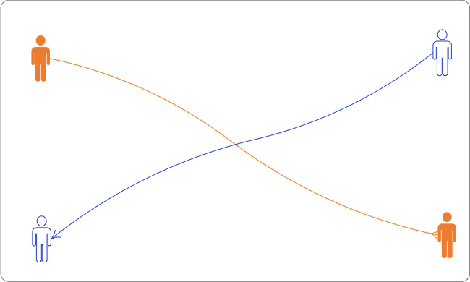
\includegraphics[width=6cm]{./png/2-monks.png}
    \end{center}

    Because both monks are continuously moving on the same path from opposite ends, they must meet at some point between 8AM and noon. At that moment, they are at exactly the same spot on the mountain.

    This means that the real monk was at that exact same spot at the same time on both days — once while going up, and once while going down.
\end{soln}

\begin{remark*}
    This result is an application of the \textbf{Intermediate Value Theorem}. Imagine a continuous function \( f(t) \) representing the difference in height between the real monk (going up) and the phantom monk (coming down). At 8AM, \( f(0) > 0 \), and at noon, \( f(4) < 0 \). Since the function is continuous, it must cross zero at some time between — meaning they are at the same height at that moment. This classic problem is often one of the earliest intuitive applications of the IVT in a geometric setting.
\end{remark*}


\begin{example}[Sum of Reciprocals of Consecutive Products (B)]\label{example:sum-of-consecutive-reciprocals}
    Determine the value of
    \[
        \frac{1}{1 \times 2} + \frac{1}{2 \times 3} + \frac{1}{3 \times 4} + \cdots + \frac{1}{99 \times 100}.
    \]
    \index{Telescoping Sums} \index{Reciprocals} \index{Consecutive Integers}
\end{example}

\begin{analysis*}
    Students, even if armed with a calculator, will see that this is hard to evaluate by determining the decimal value of each fraction:
    \[
        \frac{1}{1 \times 2} = 0.5,\quad \frac{1}{2 \times 3} = 0.1666\ldots
    \]
    Instead of calculating decimal values, we \textbf{search for a pattern}. Each denominator is a product of two consecutive integers: \( (1 \times 2), (2 \times 3), (3 \times 4), \ldots, (99 \times 100) \). 
    Since the numerator is always 1, and the denominator is a product of two consecutive integers, we can re-write each term using differences of reciprocals:
    \[
        \frac{1}{1 \times 2} = \frac{2 - 1}{1 \times 2} = \frac{1}{1} - \frac{1}{2},
    \]
    \[
        \frac{1}{2 \times 3} = \frac{3 - 2}{2 \times 3} = \frac{1}{2} - \frac{1}{3},
    \]
    \[
        \frac{1}{3 \times 4} = \frac{4 - 3}{3 \times 4} = \frac{1}{3} - \frac{1}{4},
    \]
    \[
        \vdots
    \]
    \[
        \frac{1}{99 \times 100} = \frac{100 - 99}{99 \times 100} = \frac{1}{99} - \frac{1}{100}.
    \]
\end{analysis*}

\begin{soln}[Using a telescoping sum]\ \\\indent
    In other words, each fraction is a \textbf{difference of reciprocals of consecutive integers}.  
    So, the entire sum becomes:
    \[
        \left( \frac{1}{1} - \frac{1}{2} \right) + \left( \frac{1}{2} - \frac{1}{3} \right) + \left( \frac{1}{3} - \frac{1}{4} \right) + \cdots + \left( \frac{1}{99} - \frac{1}{100} \right).
    \]
    Notice that the middle terms cancel out:
    \[
        \frac{1}{1} - \cancel{\frac{1}{2}} + \cancel{\frac{1}{2}} - \cancel{\frac{1}{3}} + \cancel{\frac{1}{3}} - \cancel{\frac{1}{4}} + \cdots + \cancel{\frac{1}{99}} - \frac{1}{100}.
    \]
    We're left with:
    \[
        \frac{1}{1} - \frac{1}{100} = \frac{100 - 1}{100} = \frac{99}{100}.
    \]
\end{soln}

\begin{remark*}
    The \emph{sum of differences principle} is used here to telescope the series and cancel out the interior terms. This is a classic and elegant example of how algebraic manipulation reveals a simple structure hidden in a long expression.
\end{remark*}


\begin{example}[Shortest Path to the River and Back (B)]\label{example:shortest-reflection-path}
    Elizabeth went on an outdoor trip. To make dinner she needed to gather wood at point \( A \), then she went to the river bank to take some water, and then she returned to the picnic site at point \( B \). What would be the shortest distance that she can travel to complete all her tasks?
    \index{Triangle Inequality} \index{Reflection} \index{Minimum Distance} \index{Symmetry Line}
\end{example}

\begin{analysis*}
    At first, it seems impossible to determine where on the river bank (point \( C \)) Elizabeth should go in order to make \( AC + CB \) as short as possible. But let's \emph{observe what information is given}.
\end{analysis*}

\begin{soln}[Reflecting for shortest distance]\ \\\indent
    The river bank is a \textbf{straight line}. Let's reflect point \( B \) over the river bank to a point \( B' \). Point \( B' \) is called the \emph{mirror image} of \( B \), and the river bank is the \emph{line of symmetry}.

    \begin{center}
        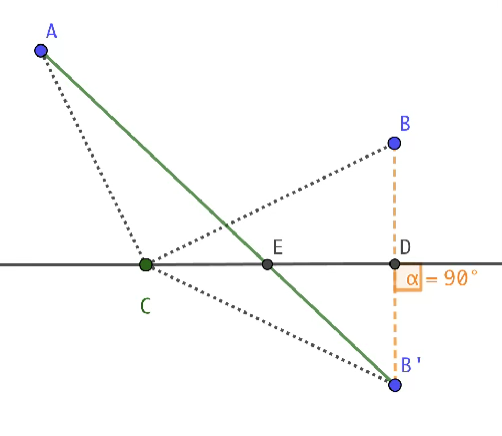
\includegraphics[width=6cm]{./png/elizabeth.png}
    \end{center}

    If we can prove that \( CB = CB' \) (which makes intuitive sense because of the reflection), then
    \[
        AC + CB = AC + CB' \ge AB',
    \]
    where the inequality comes from the triangle inequality.

    Why does \( AB' \) matter? Because it depends only on \( A \) and \( B \), and regardless of where point \( C \) lies, it allows us to minimize the total distance by aligning \( C \) with the segment \( AB' \) along the river bank.

    \textbf{Solution:} Using \textit{reflection over a line} (a type of geometry transformation), we observe the following:

    \begin{itemize}[topsep=0pt, itemsep=2pt]
        \item \( BD = DB' \), and \( \angle CDB = \angle CDB' = 90^\circ \)
        \item \( \triangle CBD \cong \triangle CB'D \) (by Angle-Side-Angle congruence)
        \item Hence, \( CB = CB' \)
    \end{itemize}

    Therefore,
    \[
        AC + CB = AC + CB' \ge AB',
    \]
    and the equality occurs when \( C \) coincides with point \( E \), the intersection of line segment \( AB' \) with the river bank.

\end{soln}

\begin{remark*}
    In this example, the \emph{triangle inequality} is used together with the \emph{reflection} over the line of symmetry (river bank) to find the shortest path. The idea is to reduce the broken path \( A \to C \to B \) into a straight segment \( A \to B' \) by choosing point \( C \) optimally.
\end{remark*}


\begin{example}[Topological Invariance Puzzle (M)]\label{example:box-topological-matching}
    Can you connect each small box \( A, B, C \) on the top with the same-letter box on the bottom with paths that do not cross one another, nor leave the boundaries of the large box?
    \index{Topology} \index{Topological Invariant} \index{Path Deformation}
\end{example}

\begin{center}
    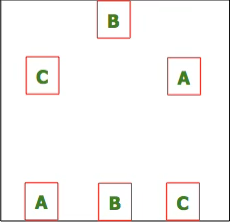
\includegraphics[width=2.5cm]{./png/3-houses.png}
\end{center}

\begin{analysis*}
    At first glance, this problem seems impossible to solve. You may not recall any similar problem to help you get started. The troublemaker appears to be the path that connects the two \( B \) boxes — it seems difficult to avoid intersecting paths.
\end{analysis*}

\begin{soln}[Bending with topological equivalence]\ \\\indent
    Let’s consider the following two ideas:
    \begin{itemize}[topsep=0pt, itemsep=2pt]
        \item The path linking the two \( B \) boxes does \emph{not} have to be a straight line.
        \item The \textit{working backwards} strategy can help — we can try to create a configuration where the connections already exist and then morph it into the original layout.
    \end{itemize}
    
    \textbf{Step-by-step Construction:}
    \begin{enumerate}[label=(\arabic*), itemsep=2pt]
        \item Redraw a configuration where the top \( A \) and \( C \) boxes are swapped.
        \item Connect the pairs: \( A \) to \( A \), \( B \) to \( B \), and \( C \) to \( C \), with simple vertical paths. This is a valid non-crossing configuration.
        \item Move the top \( C \) box into the left column, \textit{bending} the path between the two \( B \) boxes to avoid crossing with the \( C \) path.
        \item Similarly, push the top \( C \) box into the right column, and bend the paths for \( B \) and \( A \), so that \textbf{none} of the three connections intersect.
    \end{enumerate}

    \begin{center}
        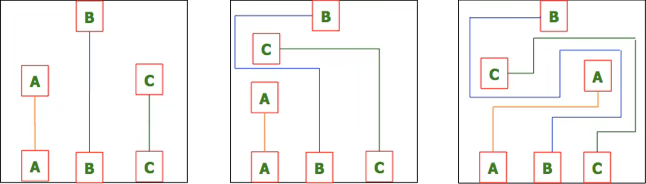
\includegraphics[width=8.5cm]{./png/3-houses-2.png}
    \end{center}

    \textbf{We are done!}
\end{soln}

\begin{remark*}
    Here, the paths can be bent, stretched, or deformed, but not broken — and they must remain inside the large box. This is an application of a \emph{topological property} or \emph{topological invariant}, which allows us to map the original problem to an equivalent one by continuous deformation. This principle often appears in puzzles involving connectivity and spatial constraints.
\end{remark*}


\begin{example}[Pythagorean Theorem — Visual Proof (E)]\label{example:pythagorean-visual}
    \textbf{Pythagorean Theorem:} In a right triangle, the square of the hypotenuse (the side opposite the right angle) is equal to the sum of the squares of the other two sides.
    \index{Pythagorean Theorem} \index{Visual Proof} \index{Geometry – Area Decomposition}
\end{example}

\begin{analysis*}
    This is one of the most famous theorems in geometry. Instead of algebraic manipulation, we can explore it through area-based reasoning by arranging right triangles in different configurations to derive the identity \( c^2 = a^2 + b^2 \).
\end{analysis*}

\begin{soln}[Solution 1 — Rearranged Squares]\ \\\indent
    On the left diagram, four right triangles with side lengths \( a, b, c \) and a square with side length \( c \) form a large square.  
    On the right diagram, the same four triangles are rearranged, and the remaining uncovered region consists of two smaller squares with areas \( a^2 \) and \( b^2 \).  
    \begin{center}
        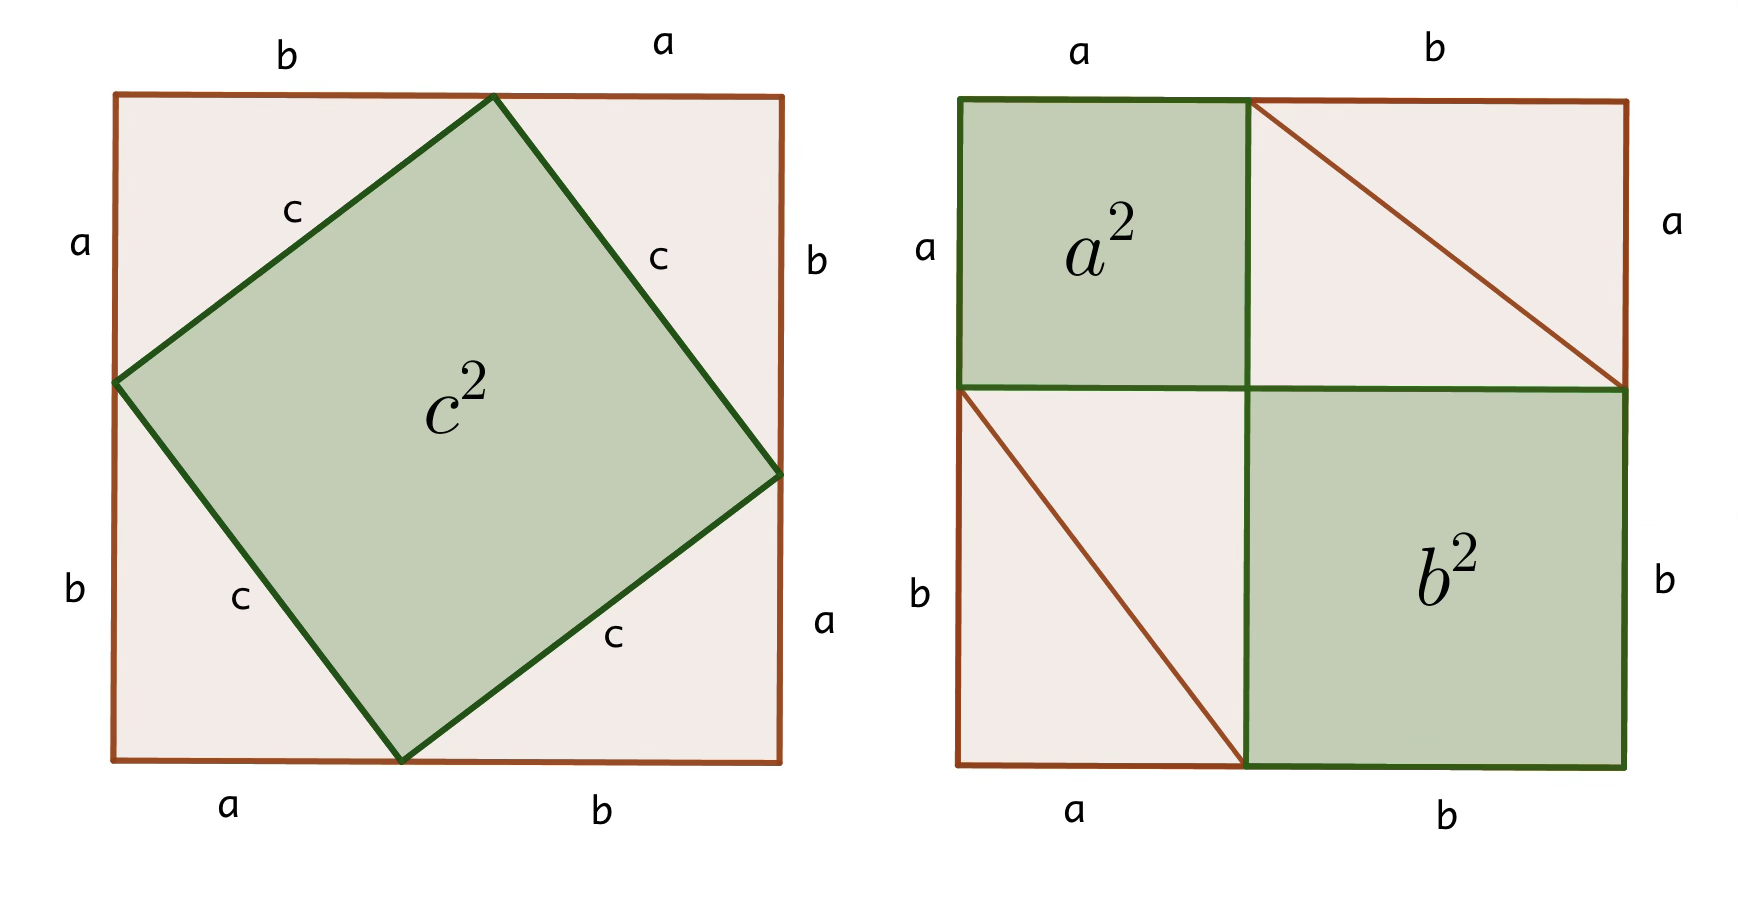
\includegraphics[width=8cm]{./png/pythagorean-1.png}
    \end{center}

    \[
        \text{So,} \quad c^2 = a^2 + b^2
    \]
\end{soln}

\begin{soln}[Solution 2 — Subtraction Method]\ \\\indent
    In the lower diagram, a square of side length \( c \) is made from four right triangles with legs \( a, b \) and hypotenuse \( c \), and a central square with side length \( b - a \).  
    \begin{center}
        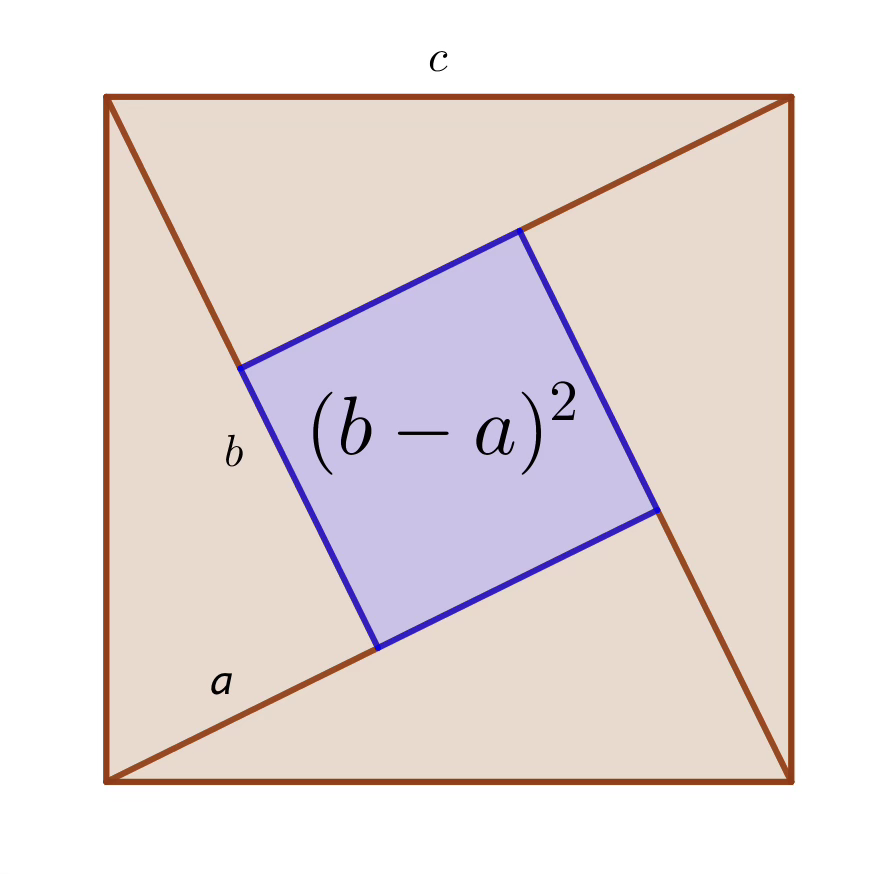
\includegraphics[width=4cm]{./png/pythagorean-2.png}
    \end{center}

    Therefore:
    \[
        (b - a)^2 + 4 \cdot \tfrac{1}{2} ab = c^2 \Rightarrow (b - a)^2 + 2ab = c^2
    \]
    Expanding:
    \[
        b^2 - 2ab + a^2 + 2ab = c^2 \Rightarrow a^2 + b^2 = c^2
    \]
\end{soln}

\begin{remark*}
    In both solutions, a \emph{visual proof} is used to provide insight. The \emph{divide-and-conquer principle} appears here: a geometrical figure is decomposed into known parts to calculate the total area and derive the identity. These strategies are especially valuable in reasoning about geometry without relying solely on algebra.
\end{remark*}


\begin{example}[Inequality via Geometric Area Comparison (E)]\label{example:inequality-area}
    For any real numbers \( a, b \geq 0 \):
    \[
        a^2 + b^2 \geq 2ab
    \]
    \index{Inequality} \index{AM–GM Inequality} \index{Geometry – Area Comparison}
\end{example}

\begin{analysis*}
    This is a trivial inequality that can be derived from the identity \( (a - b)^2 \geq 0 \).  
    But visualizing it geometrically offers more insight than simply manipulating symbols.
\end{analysis*}

\begin{soln}[Solution — Area Comparison]\ \\\indent
    Algebra — or algebraic notation — is powerful in both describing problems and providing short solutions.  
    However, it does not always help students to grasp the underlying insight.
    \begin{center}
        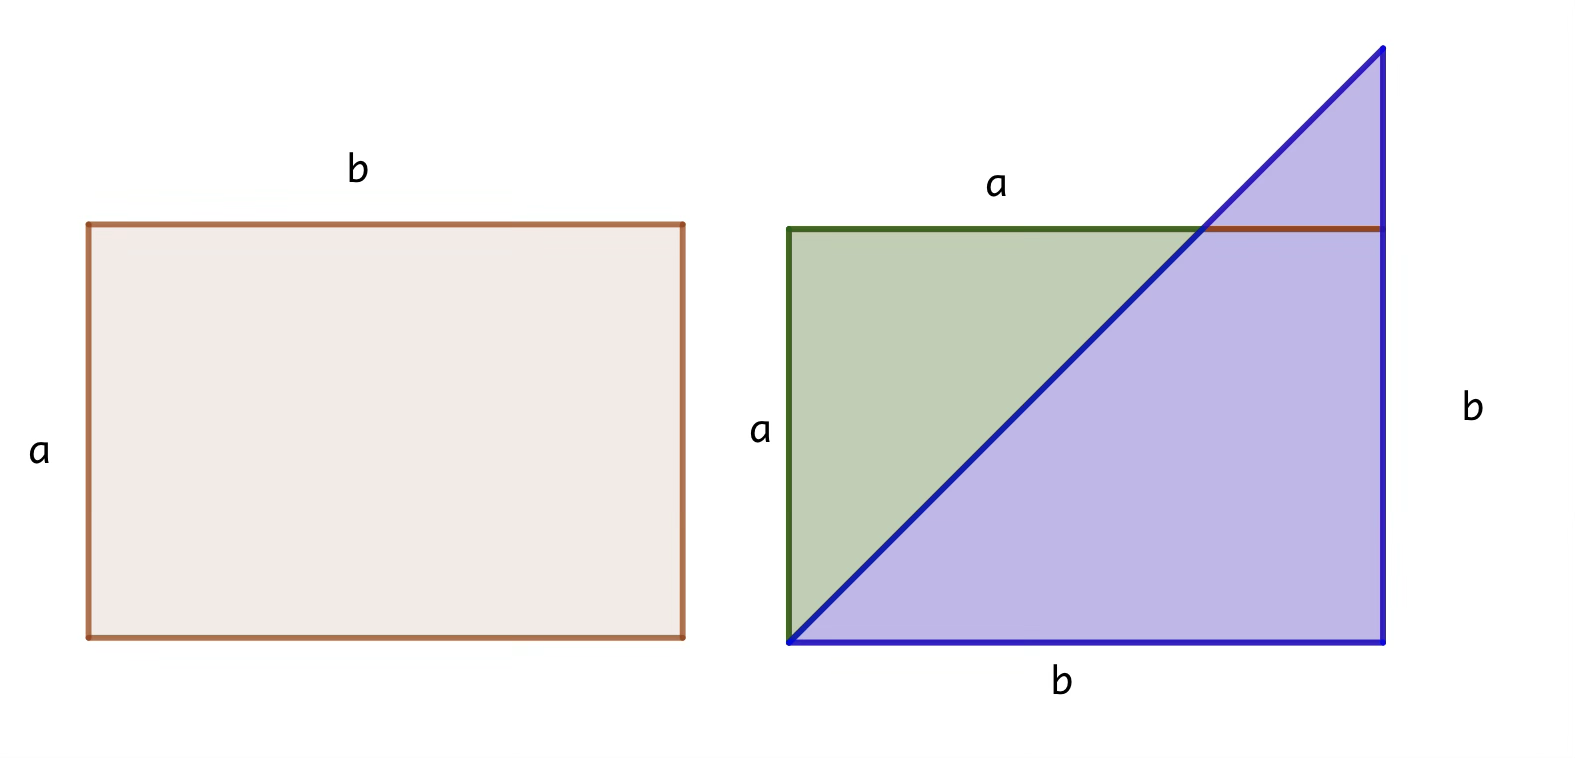
\includegraphics[width=8cm]{./png/simple-inequality.png}
    \end{center}

    Assume without loss of generality that \( b \geq a \). In the diagrams:
    \begin{itemize}[topsep=0pt, itemsep=2pt]
        \item The left figure is a rectangle with side lengths \( a \) and \( b \), hence area \( ab \).
        \item The right figure consists of two isosceles right triangles with legs \( a, b \), so their combined area is:
        \[
            \frac{1}{2}a^2 + \frac{1}{2}b^2
        \]
    \end{itemize}

    Since the rectangle fits strictly inside the two triangles:
    \[
        ab \leq \frac{1}{2}a^2 + \frac{1}{2}b^2 \Rightarrow 2ab \leq a^2 + b^2
    \]
\end{soln}

\begin{remark*}
    This proof shows a very interesting concept of how to visualize the relationship between area and side length — in particular, how comparing a rectangle and two triangles helps us interpret the inequality \( a^2 + b^2 \geq 2ab \).  
    This reflects a geometric insight behind the classic AM–GM inequality.
\end{remark*}

\begin{example}[Subset Count — Binary Representation and Tree (M)]\label{example:subset-binary-tree}
    Prove that the set \( \{1, 2, \dots, 10\} \) has exactly \( 2^{10} \) subsets.
    \index{Subsets} \index{Binary Representation} \index{Binary Tree} \index{Equivalent Problem Formulation}
\end{example}

\begin{analysis*}
    Let’s think about how to count the total number of subsets. Listing subsets by their sizes offers some insight, but we need a more systematic way to generate all possibilities. Two elegant constructions—one using a binary tree, the other using binary numbers—will help.
    What can be the subsets of \( \{1, 2, \dots, 10\} \)? Let’s list a few of them:
    \begin{itemize}[topsep=0pt, itemsep=2pt]
        \item Subsets that have zero elements: \( \{\} \). There is 1 of them.
        \item Subsets that have 1 element: \( \{1\}, \{2\}, \dots, \{10\} \). There are 10 of them.
        \item Subsets that have 2 elements: \( \{1,2\}, \{1,3\}, \dots, \{9,10\} \). There are \( \binom{10}{2} = 45 \) of them.
        \item Subsets that have 9 elements: there are \( \binom{10}{9} = 10 \) of them.
        \item Subsets that have 10 elements: \( \{1, 2, \dots, 10\} \). There is 1 of them.
    \end{itemize}

    It is not obvious how we can find the total number of subsets. The solutions below show two \textit{different equivalent ways to formulate the problem.}
\end{analysis*}

\begin{soln}[Solution 1]\ \\\indent
    Let’s draw a tree as shown in the diagram below.

    For each subset composed of the elements \( 1, 2, \dots, 10 \), there are two additional branches depending on whether a number is in the subset or not. In other words, the number of leaves of the tree equals the number of possible subsets.

    It is easy to see that the number of leaves is:
    \[
        2 \times 2 \times \dots \times 2 = 2^{10}
    \]

    \begin{center}
        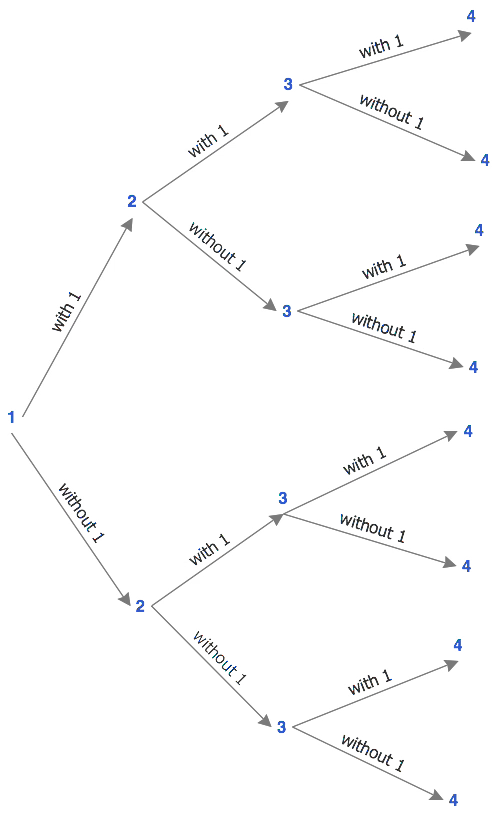
\includegraphics[width=6cm]{./png/subsets.png}
    \end{center}
\end{soln}

\begin{soln}[Solution 2]\ \\\indent
    This solution is more subtle.

    For each subset, let’s associate a 10-digit binary number. Each digit at position \( n = 1, 2, \dots, 10 \) is 1 if the number \( n \) is in the subset, and 0 otherwise.

    For example:
    \begin{itemize}[topsep=0pt, itemsep=2pt]
        \item If the subset is \( \{1, 4, 6\} \), then the number is 1001010000.
        \item If the subset is \( \{9, 10\} \), then the number is 0000000011.
    \end{itemize}

    These numbers are all possible base-2 numbers with 10 digits: from 0000000000 to 1111111111. That's exactly:
    \[
        2^{10} \text{ binary numbers}.
    \]
\end{soln}

\begin{remark*}
    \textbf{Note.} These solutions are examples of how to \textit{formulate a problem to map it to an equivalent one}, perhaps easier to solve or already known.
    \begin{itemize}[topsep=0pt, partopsep=0pt, itemsep=0pt]
        \item The first solution is based on \textit{properties of a binary tree}.
        \item The second solution is based on the \textit{representation of integers in base-2}.
    \end{itemize}
\end{remark*}

\noindent\rule{16.5cm}{0.4pt}

\section{Exercises}

\begin{exercise}[Chessboard Parity – Domino Tiling]\label{example:chessboard-domino-tiling}
    Danny the Hooligan cuts the \textbf{top-left} and \textbf{bottom-right} squares out of an \( 8 \times 8 \) chessboard.  
    He challenges Kevin the Smart to tile the remaining board using \(1 \times 2\) dominoes.  
    Can Kevin the Smart do it?
    \index{Chessboard Tiling} \index{Parity Argument} \index{Domino Tilings}
\end{exercise}

\begin{hint*}
    Try coloring the board like a regular chessboard. What color are the two corners that are removed? Then think about how each domino must cover one black and one white square.
\end{hint*}

\begin{exercise}[Dividing a Square into \( n \) Smaller Squares (M)]\label{example:square-into-smaller-squares}
    Is it possible to cut a square into:
    \begin{itemize}[topsep=0pt, itemsep=2pt]
        \item 6 squares (not necessarily the same size)?
        \item 7 squares (not necessarily the same size)?
        \item 8 squares (not necessarily the same size)?
    \end{itemize}
    \index{Dissection Problems} \index{Geometric Construction}
\end{exercise}

\begin{hint*}
    Try starting from a known dissection—for example, dividing a square into 4 or 9 smaller squares. Can you modify or add squares to increase the total count to 6, 7, or 8? Consider whether a recursive method or a visual adjustment works.
\end{hint*}

\begin{exercise}[Digit Sum and Perfect Squares (M)]\label{example:digit-sum-perfect-square}
    A number has as digits: 2000 ones, 2000 twos, and all other digits are zeros.  
    Can that number be a perfect square?
    \index{Divisibility} \index{Digit Sums} \index{Perfect Squares}
\end{exercise}

\begin{hint*}
    Consider the sum of the digits of the number. What does divisibility by 3 or 9 tell you about whether a number can be a perfect square? Recall that if a perfect square is divisible by 3, then it must be divisible by 9.
\end{hint*}

\begin{exercise}[Shortest Route via Reflection (B)]\label{example:shortest-path-reflection}
    Elizabeth was at point \( F \) on a clearcutting patch shaped like an acute angle.  
    She needed to go to the green tree line to gather wood, then to the blue river bank to fetch water, and then return to the fireplace at point \( F \).  

    How can she make the shortest trip?
    \index{Shortest Path} \index{Reflection} \index{Geometric Transformations}
\end{exercise}

\begin{center}
    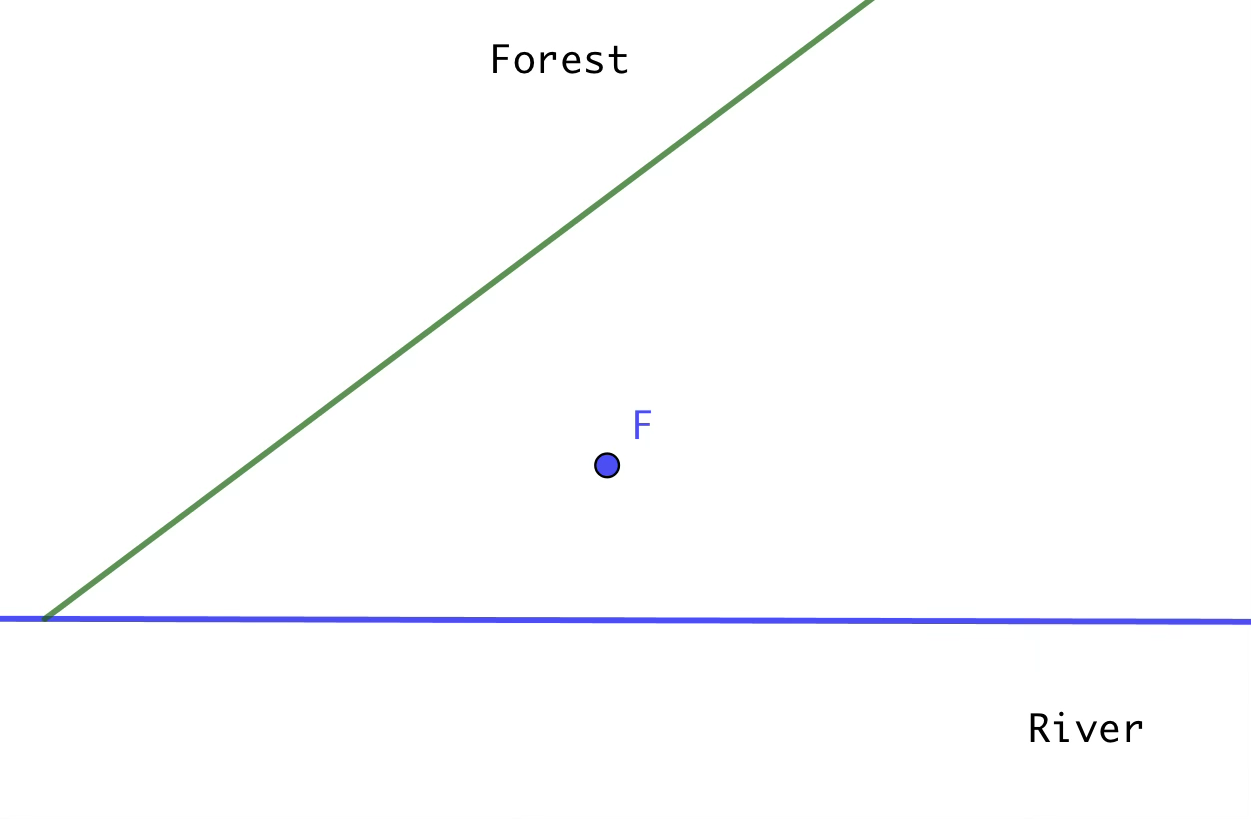
\includegraphics[width=6cm]{./png/elizabeth-2.png}
\end{center}

\begin{hint*}
    Let \( A \) be a point on the green tree line and \( B \) a point on the blue river bank.  
    Try reflecting the point \( F \) over both lines and consider the straight-line path from one reflection to another.  
    Which point along the tree line should Elizabeth first reach so that the entire path \( F \to A \to B \to F \) is minimized?
\end{hint*}

\begin{exercise}[Infinite Pizza Staircase (A)]\label{example:infinite-pizza-staircase}
    The fast-talking Donkey went up a long spiral staircase.  
    On the first step, Donkey found a whole round pizza. At every step afterward, he found half of what he got in the previous step.

    Is it possible that at some point the total amount of pizza Donkey got is more than 2 pizzas?
    \index{Geometric Series} \index{Infinity Paradox} \index{Series Convergence}
\end{exercise}

\begin{hint*}
    Try drawing the pizzas Donkey gets after each step:  
    1, \( \frac{1}{2} \), \( \frac{1}{4} \), \( \frac{1}{8} \), and so on.  

    What kind of sequence is this? Can you find a formula to compute the total amount Donkey gets after \( n \) steps?  
    Is this total ever more than 2 pizzas?
\end{hint*}

\begin{exercise}[Shortest Path on a Cube (A)]\label{example:bug-cube-shortest-path}
    A bug sits on the vertex \( A \) of a cube. It wants to crawl along the surface of the cube to the opposite vertex \( B \).  

    What is the shortest path it can take?
    \index{Unfolding Cubes} \index{3D to 2D Reduction} \index{Shortest Path on Surface}
\end{exercise}

\begin{center}
    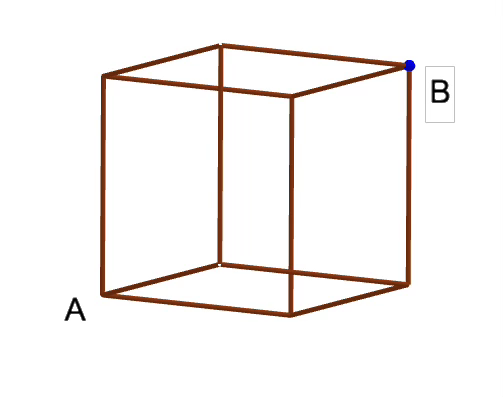
\includegraphics[width=3cm]{./png/cube.png}
\end{center}

\begin{hint*}
    Try unfolding the cube into a flat 2D net that includes both points \( A \) and \( B \). The shortest path will become a straight line between those two points in the unfolded diagram.
\end{hint*}


\begin{exercise}[Infinitely Nested Radical]\label{example:infinite-nested-radical}
    Determine the value of 
    \[
        \sqrt{2 + \sqrt{2 + \sqrt{2 + \sqrt{2 + \cdots}}}}.
    \]
    \index{Infinite Radicals} \index{Quadratic Equation from Nesting}
\end{exercise}

\begin{hint*}
    Let \( x \) be the value of the entire expression.  
    Notice that the expression inside the square root also begins with \( 2 + \sqrt{2 + \cdots} \), which is again \( x \).  
    Use this observation to write an equation in terms of \( x \), then solve it.

    If you obtain more than one solution fromt the equation, which one is correct?
\end{hint*}


\begin{exercise}[Determine the Remainder (C)]\label{example:remainder-divisibility}
    What is the remainder when 
    \[
        n = \underbrace{20132013\ldots2013}_{\text{2013 times}}
    \]
    is divided by \(333,\!333\)?
    \index{Divisibility} \index{Prime Factorization} \index{Remainder}
\end{exercise}

\begin{hint*}
    What is the prime factorization of \(333,\!333\)?  
    Try to verify whether \(n\) is divisible by each of its prime factors one by one.  
    Use rules for divisibility by \(7\), \(11\), \(13\), and \(37\), including alternating block subtraction and sum methods.  
    If \(n\) is divisible by all prime factors of \(333,\!333\), what must the remainder be?
\end{hint*}


\begin{exercise}[The Missing Dollar (E)]\label{example:missing-dollar}
    Three men went to a pub during happy hour, which was advertised to cost \$9 per person. After an hour, they each gave the waitress \$10, for a total of \$30, and asked her to bring back the change.  

    She went to the cashier and learned that the actual charge was only \$25 for a group of three.  

    Feeling lucky, she gave \$25 to the cashier, then returned and gave each man \$1 back. She secretly kept \$2 for herself.  

    Now each man paid \$9, for a total of \$27. The waitress kept \$2.  

    What happened to the missing dollar?
    \index{Trick Questions} \index{Paradox}
\end{exercise}

\begin{hint*}
    Carefully track where the money goes. Does it make sense to add what the men paid and what the waitress kept? Try verifying the flow of money from the original \$30.
\end{hint*}

\noindent\rule{16.5cm}{0.4pt}

\section{Puzzle}

\begin{otherlanguage*}{russian}

\begin{puzzle}[Linguistic Challenge – NACLO 1.10 (M)]\label{example:naclo-tajik}
    Tajik is an Indo-European language related most closely to Farsi (Persian). Most literature in Tajik uses a version of the Cyrillic script (used also in Russian, Ukrainian, Bulgarian, etc.). You do not need to read Cyrillic to solve this puzzle—just use logic.

    Below are three phrases from the Tajik language and their English translations:

    \begin{center}
        \begin{tabular}{ll}
            дустии хуби ҳамсояи шумо & a good friend of your neighbor \\
            ҳамсояи дустии хуби шумо & a neighbor of your good friend \\
            ҳамсояи хуби дустии шумо & a good neighbor of your friend \\
        \end{tabular}
    \end{center}

    Your task is to determine the English translation of each of the following four Tajik words. The possible meanings are: \textbf{``good,'' ``friend,'' ``neighbor,''} and \textbf{``your.''}

    \begin{center}
        \begin{tabular}{ll}
            дустии   & friend \\
            хуби     & good \\
            ҳамсояи  & neighbor \\
            шумо     & your \\
        \end{tabular}
    \end{center}
    \index{Linguistics} \index{Deductive Reasoning}
\end{puzzle}

\begin{soln}\ \\\indent
    Since all three Tajik sentences end with \textit{шумо}, and all English translations end with “your [noun],” we conclude:
    \[
        \text{шумо} = \textbf{your}
    \]
    
    Now compare the word orders. Consider:
    \begin{itemize}[topsep=0pt, partopsep=0pt, itemsep=2pt]
        \item Line 1: \texttt{дустии хуби ҳамсояи шумо} = a good friend of your neighbor
        \item Line 2: \texttt{ҳамсояи дустии хуби шумо} = a neighbor of your good friend
        \item Line 3: \texttt{ҳамсояи хуби дустии шумо} = a good neighbor of your friend
    \end{itemize}

    Track how word positions relate to the English translations. In line 1:
    \[
        \texttt{дустии} = \text{friend}, \quad \texttt{хуби} = \text{good}, \quad \texttt{ҳамсояи} = \text{neighbor}
    \]
    
    This is consistent with:
    \begin{itemize}[topsep=0pt, partopsep=0pt, itemsep=2pt]
        \item Line 2: ``a neighbor'' = \texttt{ҳамсояи} (1st word), ``of your good friend'' = rest of sentence
        \item Line 3: ``a good neighbor'' = \texttt{ҳамсояи хуби}, meaning \texttt{хуби} = good
    \end{itemize}

    \[
        \begin{aligned}
            \text{дустии} & = \text{friend} \\
            \text{хуби} & = \text{good} \\
            \text{ҳамсояи} & = \text{neighbor} \\
            \text{шумо} & = \text{your}
        \end{aligned}
    \]
\end{soln}

\begin{remark*}
    This puzzle tests structural reasoning and logical deduction using relative word order. The word \texttt{шумо} is clearly identifiable due to its fixed position in every sentence. Comparing shifts in word positions with changes in the English phrases reveals each word's meaning through consistent patterns.
\end{remark*}

\end{otherlanguage*}

\end{document}